% Created 2014-04-24 Thu 17:56
\documentclass[bigger]{beamer}
\usepackage[utf8]{inputenc}
\usepackage[T1]{fontenc}
\usepackage{fixltx2e}
\usepackage{graphicx}
\usepackage{longtable}
\usepackage{float}
\usepackage{wrapfig}
\usepackage{soul}
\usepackage{textcomp}
\usepackage{marvosym}
\usepackage{wasysym}
\usepackage{latexsym}
\usepackage{amssymb}
\usepackage{hyperref}
\tolerance=1000
\mode<beamer>{\usetheme[compress]{Berlin}}
\usepackage{multirow}
\setbeamertemplate{footline}
  {%
    \begin{beamercolorbox}[colsep=1.5pt]{upper separation line foot}
    \end{beamercolorbox}
    \begin{beamercolorbox}[ht=2.5ex,dp=1.125ex,%
      leftskip=.3cm,rightskip=.3cm plus1fil]{author in head/foot}%
      \leavevmode{\usebeamerfont{author in head/foot}\insertshortauthor}%
      \hfill%
      {\usebeamerfont{institute in head/foot}\usebeamercolor[fg]{institute in head/foot}\insertshortinstitute}%
    \end{beamercolorbox}%
    \begin{beamercolorbox}[ht=2.5ex,dp=1.125ex,%
      leftskip=.3cm,rightskip=.3cm plus1fil]{title in head/foot}%
      {\usebeamerfont{title in head/foot}\insertshorttitle}%
      \hfill%
      {\usebeamerfont{frame number}\usebeamercolor[fg]{frame number}\insertframenumber~/~\inserttotalframenumber}
    \end{beamercolorbox}%
    \begin{beamercolorbox}[colsep=1.5pt]{lower separation line foot}
    \end{beamercolorbox}
  }
\makeatother


%----------------------------------------------------------------------
% Define useful commands
%----------------------------------------------------------------------

\newcommand{\eejj}{\ensuremath{eejj} }
\newcommand{\enujj}{\ensuremath{e\nu jj} }
\newcommand{\mumujj}{\ensuremath{\mu\mu jj} }
\newcommand{\munujj}{\ensuremath{\mu\nu jj} }
\newcommand{\emujj}{\ensuremath{e\mu jj} }
\newcommand{\zjets}{\ensuremath{\text{Z}^{0}}+jets }
\newcommand{\wjets}{\ensuremath{\text{W}^{\pm}}+jets }
\newcommand{\ttbar}{\ensuremath{t\bar{t}} }

\newcommand{\pt}{\ensuremath{p_{\text{T}}} }
\newcommand{\ST}{\ensuremath{S_{\text{T}}} }
\newcommand{\mee}{\ensuremath{m_{\text{ee}}} }
\newcommand{\mll}{\ensuremath{m_{\ell\ell}} }
\newcommand{\mej}{\ensuremath{m_{\text{ej}}} }
\newcommand{\mejmin}{\ensuremath{m_{\text{ej}}^{\text{min}}} }
\newcommand{\mejavg}{\ensuremath{m_{\text{ej}}^{\text{avg}}} }
% \newcommand{\mt}{\ensuremath{m_{\text{T, e}\nu}}}
\newcommand{\mtjnu}{\ensuremath{m_{\text{T, j}\nu}} }


\newcommand{\met}{\ensuremath{\not\!\!{E_{\text{T}}}} }
\newcommand{\mt}{\ensuremath{m_{\text{T, e}\nu}} }

%----------------------------------------------------------------------
% Define useful numbers
%----------------------------------------------------------------------

% Lumi info
\newcommand{\intLumi}{$19.6 \text{ fb}^{-1}$}

% MC scale factors
\newcommand{\enujjWJetsMonteCarloScaleFactor}{0.85 \pm 0.01 \text{ (stat)} \pm 0.01    \text{ (syst)}}
\newcommand{\enujjTTBarMonteCarloScaleFactor}{0.97 \pm 0.02 \text{ (stat)} \pm 0.01    \text{ (syst)}}
% \newcommand{\eejjZJetsMonteCarloScaleFactor} {0.97 \pm 0.01 \text{ (stat)} \pm 0.00004 \text{ (syst)}}
\newcommand{\eejjZJetsMonteCarloScaleFactor} {0.97 \pm 0.01 \text{ (stat)}}

\newcommand{\enujjWJetsMonteCarloScaleFactorMETRescaled}{0.95 \pm 0.02 \text{ (stat)} \pm 0.01 \text{ (syst)}}
\newcommand{\enujjTTBarMonteCarloScaleFactorMETRescaled}{1.07 \pm 0.03 \text{ (stat)} \pm 0.01 \text{ (syst)}}

\newcommand{\enujjWJetsMonteCarloScaleFactorMETandMTRescaled}{0.97 \pm 0.02 \text{ (stat)} \pm 0.01 \text{ (syst)}}
\newcommand{\enujjTTBarMonteCarloScaleFactorMETandMTRescaled}{1.08 \pm 0.03 \text{ (stat)} \pm 0.01 \text{ (syst)}}

\newcommand{\eejjZControlRegionContamination}{4\%}

% Electron scale factors
\newcommand{\electronRecoDataMCScaleFactor}{0.98}
\newcommand{\electronRecoDataMCScaleFactorRelUnc}{1.5}
\newcommand{\electronRecoDataMCScaleFactorSqr}{0.96}

% GEN-level cross-sections (not yet rescaled) 
\newcommand{\wjetsXSection}{37509.0 pb}
\newcommand{\zjetsXSection}{3503.71 pb}
\newcommand{\ttbarXSection}{234 pb}
\newcommand{\stopSChannelXSection}{5.55 pb}
\newcommand{\stopTChannelXSection}{87.1 pb}
\newcommand{\stopTWChannelXSection}{22.2 pb}
\newcommand{\wwXSection}{57.1 pb} % THESE NEED TO BE UPDATED!!!
\newcommand{\wzXSection}{32.3 pb} % THESE NEED TO BE UPDATED!!!
\newcommand{\zzXSection}{8.26 pb} % THESE NEED TO BE UPDATED!!!

% QCD contributions at limit of the analysis
\newcommand{\percentQCDatEEJJLimit}{1\%}
\newcommand{\percentQCDatENuJJLimit}{3\%}

% Closure test contamination
\newcommand{\percentContaminationClosureTest}{5\%}
\newcommand{\percentContaminationClosureTestFinal}{55\%}

% Closure test (low-ST) results
\newcommand{\closureTestLowSTPredicted}{13100}
\newcommand{\closureTestLowSTPredictedUnc}{400}
\newcommand{\closureTestLowSTObserved}{12100}
\newcommand{\closureTestLowSTObservedUnc}{400}
\newcommand{\closureTestLowSTRatio}{1.08}
\newcommand{\closureTestLowSTRatioUnc}{0.05}

% Closure test (mid-ST) results
\newcommand{\closureTestMidSTPredicted}{877}
\newcommand{\closureTestMidSTPredictedUnc}{46.7}
\newcommand{\closureTestMidSTObserved}{600}
\newcommand{\closureTestMidSTObservedUnc}{53}
\newcommand{\closureTestMidSTRatio}{1.46}
\newcommand{\closureTestMidSTRatioUnc}{0.15}

% QCD systematic uncertainty
\newcommand{\qcdSystematicUncertaintyPerEle}{30\%}
\newcommand{\qcdSystematicUncertaintyTwoEle}{60\%}

% TTbar (e-mu-jj) contamination
\newcommand{\emujjContamination}{2\%}
\newcommand{\emujjRecoScaleFactor}{0.974  \pm 0.011 \text{ (stat)}}

% mumujj/munujj scale factors for data-driven background
\newcommand{\mumujjRecoScaleFactor}{97.5 \pm 0.4 \text{ (stat)}}
\newcommand{\munujjRecoScaleFactor}{97.2 \pm 0.5 \text{ (stat)}}

% Shape uncertainties
\newcommand{\enujjWJetsShapeUncertainty}{5.92\%}
\newcommand{\enujjTTBarShapeUncertainty}{8.17\%}
\newcommand{\eejjZJetsShapeUncertainty}{8.70\%}

% EES uncertainties
\newcommand{\electronEnergyScaleUncBarrel}{0.4\%}
\newcommand{\electronEnergyScaleUncEndcap}{4.1\%}

% EER uncertainties
\newcommand{\electronEnergyResolutionUncBarrel}{1.006}
\newcommand{\electronEnergyResolutionUncEndcap}{1.015}

% lumi uncertainty
\newcommand{\lumiUncertainty}{2.6\%}

% limits
\newcommand{\eejjObservedLimit}{1005}
\newcommand{\eejjExpectedLimit}{1030}
\newcommand{\enujjObservedLimit}{845}
\newcommand{\enujjExpectedLimit}{890}

\newcommand{\enujjObservedLimitCombined}{845}
\newcommand{\enujjExpectedLimitCombined}{932}

\newcommand{\eejjObservedLimitNoSyst}{1010}
\newcommand{\eejjExpectedLimitNoSyst}{1030}
\newcommand{\enujjObservedLimitNoSyst}{850}
\newcommand{\enujjExpectedLimitNoSyst}{895}

\newcommand{\eejjObservedLimitMuon}{1015}
\newcommand{\eejjExpectedLimitMuon}{980}
\newcommand{\enujjObservedLimitMuon}{825}
\newcommand{\enujjExpectedLimitMuon}{890}


\newcommand{\lowBetaExpectedLimit}{790}
\newcommand{\lowBetaObservedLimit}{635}

\makeatletter
\newcommand\ChangeItemFont[3]{%
\renewcommand{\itemize}[1][]{%
  \beamer@ifempty{##1}{}{\def\beamer@defaultospec{#1}}%
  \ifnum \@itemdepth >2\relax\@toodeep\else
    \advance\@itemdepth\@ne
    \beamer@computepref\@itemdepth% sets \beameritemnestingprefix
    \usebeamerfont{itemize/enumerate \beameritemnestingprefix body}%
    \usebeamercolor[fg]{itemize/enumerate \beameritemnestingprefix body}%
    \usebeamertemplate{itemize/enumerate \beameritemnestingprefix body begin}%
    \list
      {\usebeamertemplate{itemize \beameritemnestingprefix item}}
      {\def\makelabel####1{%
          {%
            \hss\llap{{%
                \usebeamerfont*{itemize \beameritemnestingprefix item}%
                \usebeamercolor[fg]{itemize \beameritemnestingprefix item}####1}}%
          }%
        }%
  \ifnum\@itemdepth=1\relax
    #1%
  \else
  \ifnum\@itemdepth=2\relax
    #2%
  \else
  \ifnum\@itemdepth=3\relax
    #3%
  \fi%
  \fi%
  \fi%
  }
  \fi%
  \beamer@cramped%
  \raggedright%
  \beamer@firstlineitemizeunskip%
}}
\makeatother

\mode<beamer>{\usecolortheme{bear}}
\mode<beamer>{\titlegraphic{\includegraphics[width=0.2\textwidth]{brown-logo}}}
\providecommand{\alert}[1]{\textbf{#1}}

\title{HCAL Reconstruction: \newline MC Correction Functions Update}
\author{Edmund Berry}
\date{Thursday, April 24, 2014}
\hypersetup{
  pdfkeywords={},
  pdfsubject={},
  pdfcreator={Emacs Org-mode version 7.8.11}}

\author[Edmund Berry]{\alert{Edmund Berry}}
\begin{document}

\maketitle


\section{Introduction}
\label{sec-1}
\subsection{Introduction}
\label{sec-1-1}
\begin{frame}
\frametitle{Introduction}
\label{sec-1-1-1}
\begin{itemize}

\item Alexandre's talk describes a method for OOT PU corrections on data
\label{sec-1-1-1-1}%

\item We would like to apply the same method for Monte Carlo
\label{sec-1-1-1-2}%

\item Procedure:
\label{sec-1-1-1-3}%
\begin{itemize}

\item Run Alexandre's ratio method on zero PU MC
\label{sec-1-1-1-3-1}%

\item Derive correction functions based on the pulse shape
\label{sec-1-1-1-3-2}%

\item Use the same definitions, fits, and methods as in data
\label{sec-1-1-1-3-3}%

\item Validate results on MC with OOT PU
\label{sec-1-1-1-3-4}%
\end{itemize} % ends low level

\item More details on the following slides
\label{sec-1-1-1-4}%
\end{itemize} % ends low level
\end{frame}
\section{Procedure}
\label{sec-2}
\subsection{Datasets}
\label{sec-2-1}
\begin{frame}
\frametitle{GEN-SIM datasets}
\label{sec-2-1-1}
\begin{itemize}

\item Consider two \texttt{GEN-SIM} datasets (no PU) at \texttt{T1\_US\_FNAL}:\\
\label{sec-2-1-1-1}%
\resizebox{0.9\textwidth}{!}{
\begin{tabular}{l|l}
\hline\hline
Dataset & Production release \\
\hline\hline
\texttt{/MinBias\_TuneZ2star\_13TeV-pythia6/Summer13-START53\_V7C-v1/GEN-SIM} & \texttt{CMSSW\_5\_3\_10\_patch2} \\
\texttt{/QCD\_Pt-1800\_TuneZ2star\_13TeV\_pythia6/Fall13-POSTLS162\_V1-v1/GEN-SIM} & \texttt{CMSSW\_6\_2\_0\_patch1} \\
\hline\hline
\end{tabular}
}

\item \texttt{QCD\_Pt-1800} dataset:
\label{sec-2-1-1-2}%
\begin{itemize}

\item \href{https://cmsweb.cern.ch/das/request?input=dataset\%3D\%2FQCD_Pt-1800_TuneZ2star_13TeV_pythia6\%2FFall13-POSTLS162_V1-v1\%2FGEN-SIM\&instance=prod\%2Fglobal}{\alert{DAS link}}
\label{sec-2-1-1-2-1}%

\item 93453 (\($\sim100$k\)) events, 95 files
\label{sec-2-1-1-2-2}%

\item HcalNoiseAnalyzer ntuples on FNAL EOS: \texttt{/eos/uscms/store/user/eberry/QCD1800MC/}
\label{sec-2-1-1-2-3}%
\end{itemize} % ends low level

\item \texttt{MinBias} dataset:
\label{sec-2-1-1-3}%
\begin{itemize}

\item \href{https://cmsweb.cern.ch/das/request?input=dataset\%3D\%2FMinBias_TuneZ2star_13TeV-pythia6\%2FSummer13-START53_V7C-v1\%2FGEN-SIM\&instance=prod\%2Fglobal}{\alert{DAS link}}
\label{sec-2-1-1-3-1}%

\item 9999424 (\($\sim10$M\)) events, 946 files
\label{sec-2-1-1-3-2}%

\item HcalNoiseAnalyzer ntuples on FNAL EOS: \texttt{/eos/uscms/store/user/eberry/MinBiasMC/}
\label{sec-2-1-1-3-3}%
\end{itemize} % ends low level
\end{itemize} % ends low level
\end{frame}
\subsection{Processing}
\label{sec-2-2}
\begin{frame}
\frametitle{No pileup processing (OLD and DONE):}
\label{sec-2-2-1}
\begin{itemize}

\item Need to process datasets to get \texttt{DIGI} and \texttt{RECO}
\label{sec-2-2-1-1}%

\item Steps needed: \\\\
\label{sec-2-2-1-2}%
\texttt{DIGI}, \texttt{L1}, \texttt{DIGI2RAW}, \texttt{HLT}, \texttt{RAW2DIGI}, \texttt{L1Reco}, \texttt{RECO}

\item Then run \texttt{HcalNoiseAnalyzer} (updated for 62X)
\label{sec-2-2-1-3}%
\begin{itemize}

\item \href{https://github.com/FHead/HcalNoiseAnalyzerCMS}{\alert{HcalNoiseAnalyzer git page}}, Maintained by noise group?
\label{sec-2-2-1-3-1}%

\item \href{http://eberry.web.cern.ch/eberry/HcalNoiseAnalyzer62X.cc.txt}{\alert{Updated .cc file for 62X}}, E. Berry
\label{sec-2-2-1-3-2}%
\end{itemize} % ends low level

\item Use \texttt{CMSSW\_6\_2\_8} to process \texttt{QCD\_Pt-1800} dataset:
\label{sec-2-2-1-4}%
\begin{itemize}

\item \href{https://raw.githubusercontent.com/edmundaberry/HcalReco/master/test/hcalNoise_fromGEN-SIM_62X_cmsDriver.sh}{\alert{cmsDriver.py command}}
\label{sec-2-2-1-4-1}%

\item \href{https://raw.githubusercontent.com/edmundaberry/HcalReco/master/test/hcalNoise\_fromGEN-SIM\_62X\_cfg.py}{\alert{Final python cfg}}
\label{sec-2-2-1-4-2}%
\end{itemize} % ends low level
\end{itemize} % ends low level
\end{frame}
\begin{frame}
\frametitle{With pileup processing (NEW and COMING)}
\label{sec-2-2-2}
\begin{itemize}

\item Need to overlay \texttt{QCD} with \texttt{MinBias}
\label{sec-2-2-2-1}%

\item Use \texttt{MixingModule} in \texttt{CMSSW\_6\_2\_8}
\label{sec-2-2-2-2}%

\item Pileup scenario: \texttt{AVE\_50\_BX\_25ns}
\label{sec-2-2-2-3}%

\item Two stages:
\label{sec-2-2-2-4}%
\begin{itemize}

\item 1) \texttt{DIGI}, \texttt{L1}, \texttt{DIGI2RAW}, \texttt{HLT}
\label{sec-2-2-2-4-1}%

\item 2) \texttt{RAW2DIGI} \texttt{L1Reco} \texttt{RECO}
\label{sec-2-2-2-4-2}%
\end{itemize} % ends low level

\item Stage 1: Done
\label{sec-2-2-2-5}%
\begin{itemize}

\item \href{https://github.com/edmundaberry/HcalReco/blob/master/test/hcalNoise_fromGEN-SIM_toGEN-SIM-RAW_62X_withMixer_cmsDriver.sh}{\alert{cmsDriver.py command}}
\label{sec-2-2-2-5-1}%

\item \href{https://github.com/edmundaberry/HcalReco/blob/master/test/hcalNoise_fromGEN-SIM_toGEN-SIM-RAW_62X_withMixer_cfg.py}{\alert{Final python cfg}}
\label{sec-2-2-2-5-2}%
\end{itemize} % ends low level

\item Stage 2: Subset done
\label{sec-2-2-2-6}%
\begin{itemize}

\item \href{https://github.com/edmundaberry/HcalReco/blob/master/test/hcalNoise_fromGEN-SIM-RAW_62X_cmsDriver.sh}{\alert{cmsDriver.py command}}
\label{sec-2-2-2-6-1}%

\item \href{https://github.com/edmundaberry/HcalReco/blob/master/test/hcalNoise_fromGEN-SIM-RAW_62X_cfg.py}{\alert{Final python cfg}}
\label{sec-2-2-2-6-2}%
\end{itemize} % ends low level

\item High PU is \alert{VERY} CPU intensive: 2 minutes/event
\label{sec-2-2-2-7}%
\end{itemize} % ends low level
\end{frame}
\begin{frame}
\frametitle{Pileup vs. No Pileup pulse shape comparison: HB}
\label{sec-2-2-3}
%% Figure
\label{sec-2-2-3-1}

\centering
Example single DIGI comparison: HB
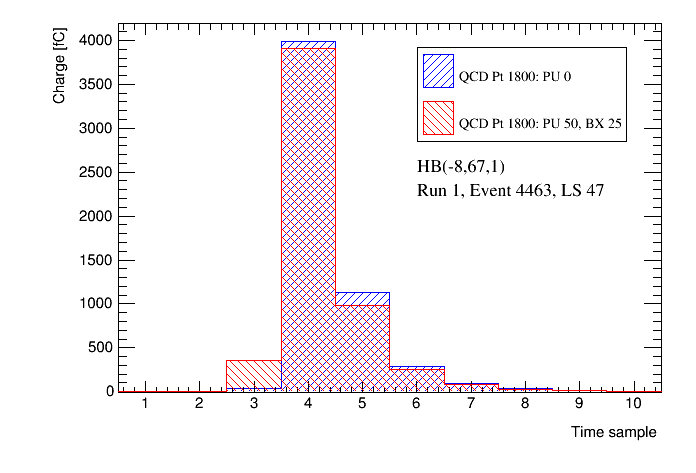
\includegraphics[width=0.6\textwidth]{fig/pulse_QCD1800MC_PU_vs_NoPU.png}
%% Text
\label{sec-2-2-3-2}
\begin{itemize}

\item As expected in TS3.  Strangeness in TS4 + TS5.
\label{sec-2-2-3-2-1}%

\item Bug in \texttt{MixingModule}?  Investigating.
\label{sec-2-2-3-2-2}%

\item More detailed results coming (HCAL DPG meeting)
\label{sec-2-2-3-2-3}%
\end{itemize} % ends low level
\end{frame}
\begin{frame}
\frametitle{Pileup vs. No Pileup pulse shape comparison: HE}
\label{sec-2-2-4}
%% Figure
\label{sec-2-2-4-1}

\centering
Example single DIGI comparison: HE
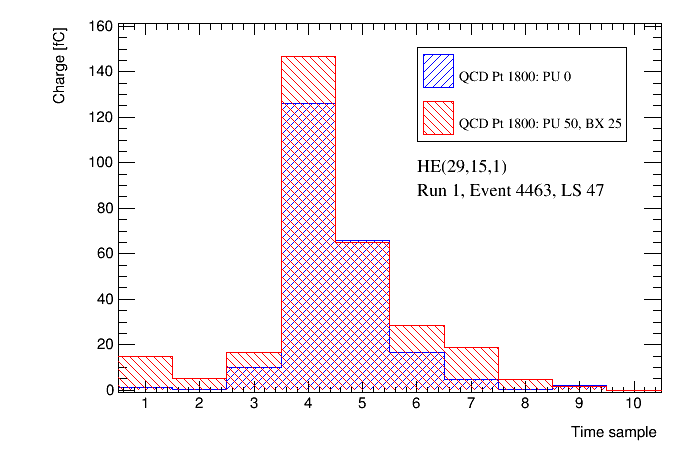
\includegraphics[width=0.6\textwidth]{fig/pulse_QCD1800MC_PU_vs_NoPU_HE.png}
%% Text
\label{sec-2-2-4-2}
\begin{itemize}

\item More or less as expected
\label{sec-2-2-4-2-1}%

\item More detailed results coming (HCAL DPG meeting)
\label{sec-2-2-4-2-2}%
\end{itemize} % ends low level
\end{frame}
\subsection{Selection}
\label{sec-2-3}
\begin{frame}
\frametitle{Selecton}
\label{sec-2-3-1}
\begin{itemize}

\item Event selection:
\label{sec-2-3-1-1}%
\begin{itemize}

\item No trigger requirement
\label{sec-2-3-1-1-1}%

\item No \texttt{OfficialDecision} requirement
\label{sec-2-3-1-1-2}%

\item \texttt{NumberOfGoodPrimaryVertices > 0}
\label{sec-2-3-1-1-3}%
\end{itemize} % ends low level

\item Channel selection:
\label{sec-2-3-1-2}%
\begin{itemize}

\item Only \texttt{HBHE} considered
\label{sec-2-3-1-2-1}%

\item Rings: HB, HE: \{17:20, 21:23, 24:25, 26:27, 28:28\}
\label{sec-2-3-1-2-2}%

\item No channels in bad channels list
\label{sec-2-3-1-2-3}%

\item \texttt{RecHit} energy > 1 GeV
\label{sec-2-3-1-2-4}%

\item Charge > 5 fC
\label{sec-2-3-1-2-5}%
\end{itemize} % ends low level

\item Analyzer code:
\label{sec-2-3-1-3}%
\begin{itemize}

\item \href{https://github.com/edmundaberry/HcalReco/blob/master/analysis/macros/analysisClass_hcalReco.C}{\alert{Git page}}
\label{sec-2-3-1-3-1}%
\end{itemize} % ends low level
\end{itemize} % ends low level
\end{frame}
\section{Results}
\label{sec-3}
\subsection{N(vertex)}
\label{sec-3-1}
\begin{frame}
\frametitle{N(vertex)}
\label{sec-3-1-1}
%% Figure
\label{sec-3-1-1-1}

\centering
Number of primary vertices: QCD sample
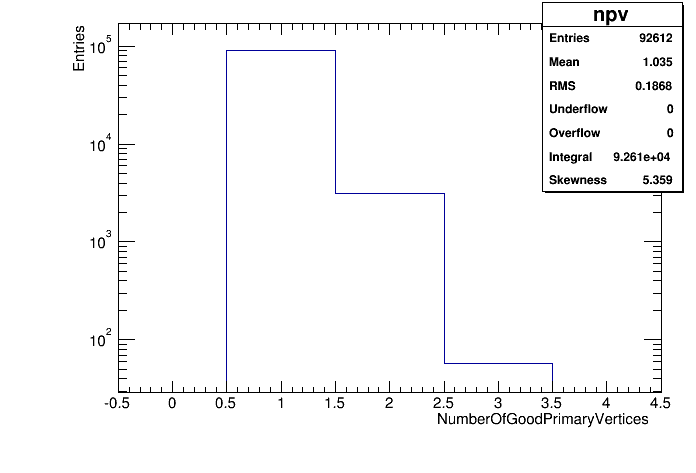
\includegraphics[width=0.6\textwidth]{fig/npv_QCD1800.png}
%% Text
\label{sec-3-1-1-2}
\begin{itemize}

\item 92612 events passing event selection
\label{sec-3-1-1-2-1}%

\item Confirms no pileup, as expected
\label{sec-3-1-1-2-2}%
\end{itemize} % ends low level
\end{frame}
\subsection{Definitions}
\label{sec-3-2}
\begin{frame}
\frametitle{Definitions}
\label{sec-3-2-1}
\begin{itemize}

\item The following plots show TProfile distributions
\label{sec-3-2-1-1}%

\item One entry per HCAL digi in the ZS-collection
\label{sec-3-2-1-2}%

\item $x$-axis corresponds to charge in TS4 [fC]
\label{sec-3-2-1-3}%

\item $y$-axis corresponds to one of several charge ratios:
\label{sec-3-2-1-4}%
\begin{itemize}

\item a\_1: charge in TS3 [fC] / charge in TS4 [fC]
\label{sec-3-2-1-4-1}%

\item a1: charge in TS5 [fC] / charge in TS4 [fC]
\label{sec-3-2-1-4-2}%

\item a2: charge in TS6 [fC] / charge in TS4 [fC]
\label{sec-3-2-1-4-3}%

\item a3: charge in TS7 [fC] / charge in TS4 [fC]
\label{sec-3-2-1-4-4}%
\end{itemize} % ends low level
\end{itemize} % ends low level
\end{frame}
\subsection{a\_1(TS4) in the QCD sample}
\label{sec-3-3}
\begin{frame}
\frametitle{a\_1(TS4) in the QCD sample}
\label{sec-3-3-1}
\begin{columns} % Columns
\label{sec-3-3-1-1}
\begin{column}{0.55\textwidth}
%% Figure
\label{sec-3-3-1-1-1}

\centering
a\_1(TS4) in HB
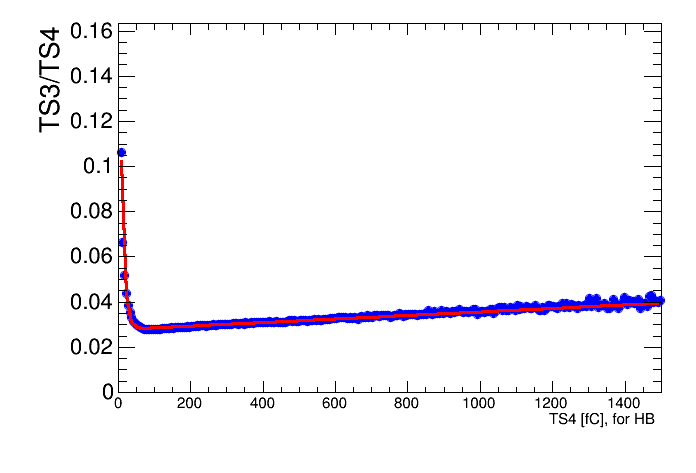
\includegraphics[width=\textwidth]{fig/a0_ring0.png}
\end{column}
\begin{column}{0.55\textwidth}
%% Figure
\label{sec-3-3-1-1-2}

\centering
a\_1(TS4) in HE 17:20
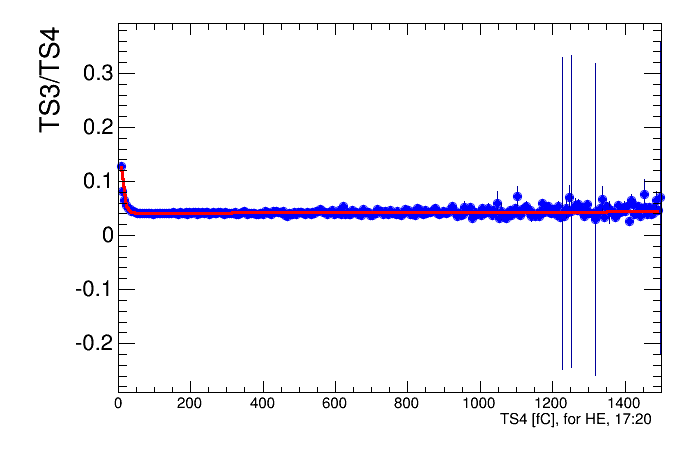
\includegraphics[width=\textwidth]{fig/a0_ring1.png}
\end{column}
\end{columns}
%% Text
\label{sec-3-3-1-2}
\begin{itemize}

\item Fit with exponential + polynomial:\\
\label{sec-3-3-1-2-1}%
\resizebox{0.8\textwidth}{!}{
\begin{equation*}
a\_1(\text{TS4}) = [0] + [1]\cdot\text{TS4} + \text{Exp}\left([2] + [3]\cdot\text{TS4}\right)
\end{equation*}
}
\end{itemize} % ends low level
\end{frame}
\subsection{a1(TS4) in the QCD sample}
\label{sec-3-4}
\begin{frame}
\frametitle{a1(TS4) in the QCD sample}
\label{sec-3-4-1}
\begin{columns} % Columns
\label{sec-3-4-1-1}
\begin{column}{0.5\textwidth}
%% Figure
\label{sec-3-4-1-1-1}

\centering
a1(TS4) in HB
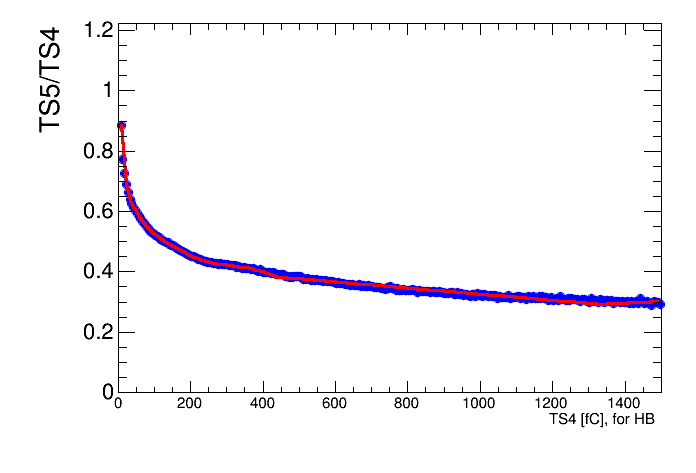
\includegraphics[width=\textwidth]{fig/a1_ring0.png}
\end{column}
\begin{column}{0.5\textwidth}
%% Figure
\label{sec-3-4-1-1-2}

\centering
a1(TS4) in HE 17:20
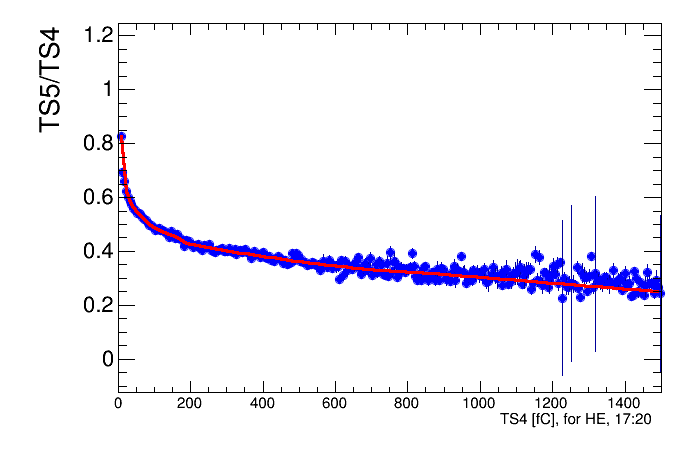
\includegraphics[width=\textwidth]{fig/a1_ring1.png}
\end{column}
\end{columns}
%% Text
\label{sec-3-4-1-2}
\begin{itemize}

\item Fit with multiple polynomials (same shape as in data)
\label{sec-3-4-1-2-1}%

\item Fit function describes the shape well
\label{sec-3-4-1-2-2}%

\item Numeric results and data comparison next slide
\label{sec-3-4-1-2-3}%
\end{itemize} % ends low level
\end{frame}
\begin{frame}
\frametitle{a1(TS4) in the QCD sample: HB}
\label{sec-3-4-2}
%% Table
\label{sec-3-4-2-1}

\begin{center}
\resizebox*{!}{0.75\textheight}{
\begin{tabular}{c|c|rcl|c}
\hline\hline
Variable & Region & \multicolumn{3}{c|}{MC value (unc. from fit)} & Data value \\ 
\hline\hline
$a_{0}$ & \multirow{5}{*}{$\text{TS4} < 28$ fC} & $1.4$ & $\pm$ & $0.00028$ & $0.73$ \\ 
$a_{1}$ & & $-0.12$ & $\pm$ & $2e-05$ & $-0.031$ \\ 
$a_{2}$ & & $0.0083$ & $\pm$ & $7.5e-07$ & $0.0012$ \\ 
$a_{3}$ & & $-0.00027$ & $\pm$ & $2.6e-08$ & $-1.3e-05$ \\ 
$a_{4}$ & & $3.4e-06$ & $\pm$ & $9.1e-10$ & $-5.5e-08$ \\ 
\hline
$b_{0}$ & \multirow{5}{*}{$28 \leq\text{TS4} < 60$ fC} & $0.84$ & $\pm$ & NA & $0.42$ \\ 
$b_{1}$ & & $-0.0078$ & $\pm$ & $2e-05$ & $0.0069$ \\ 
$b_{2}$ & & $3.7e-05$ & $\pm$ & $2.3e-07$ & $-0.00033$ \\ 
$b_{3}$ & & $1.1e-06$ & $\pm$ & $3.3e-09$ & $4.9e-06$ \\ 
$b_{4}$ & & $-1.1e-08$ & $\pm$ & $5e-11$ & $-2.4e-08$ \\ 
\hline
$c_{0}$ & \multirow{4}{*}{$60 \leq\text{TS4} < 190$ fC} & $0.76$ & $\pm$ & NA & $0.47$ \\ 
$c_{1}$ & & $-0.0042$ & $\pm$ & $5.2e-06$ & $-0.0015$ \\ 
$c_{2}$ & & $2.4e-05$ & $\pm$ & $2.2e-08$ & $4.3e-06$ \\ 
$c_{3}$ & & $-5.5e-08$ & $\pm$ & $1e-10$ & $-4.7e-09$ \\ 
\hline
$d_{0}$ & \multirow{4}{*}{$190 \leq\text{TS4} < 435$ fC} & $0.77$ & $\pm$ & NA &  $0.53$ \\ 
$d_{1}$ & & $-0.003$ & $\pm$ & $3.7e-06$  & $-0.0019$ \\ 
$d_{2}$ & & $9.1e-06$ & $\pm$ & $6.5e-09$  & $4.6e-06$ \\ 
$d_{3}$ & & $-9.7e-09$ & $\pm$ & $1.2e-11$  & $-3.8e-09$ \\ 
\hline
$e_{0}$ & \multirow{2}{*}{$435 \leq\text{TS4} < 1330$ fC} & $0.43$ & $\pm$ & NA & $0.26$ \\ 
$e_{1}$ & & $-0.0001$ & $\pm$ & $5.1e-07$ & $-1.9e-05$ \\ 
\hline
$f_{0}$ & \multirow{2}{*}{$1330 \text{ fC} \leq \text{TS4}$} & $0.43$ & $\pm$ & NA & $0.24$ \\ 
$f_{1}$ & & $5.5e-05$ & $\pm$ & $5.9e-06$ & $-3.6e-07$ \\ 
\hline\hline
\end{tabular}

}
\end{center}
\end{frame}
\begin{frame}
\frametitle{a1(TS4) in the QCD sample: HE 17:20}
\label{sec-3-4-3}
%% Table
\label{sec-3-4-3-1}

\begin{center}
\resizebox*{!}{0.75\textheight}{
\begin{tabular}{c|c|rcl|c}
\hline\hline
Variable & Region & \multicolumn{3}{c|}{MC value (unc. from fit)} & Data value \\ 
\hline\hline
$a_{0}$ & \multirow{5}{*}{$\text{TS4} < 23$ fC} & $1.5$ & $\pm$ & $0.00041$ & $0.61$ \\ 
$a_{1}$ & & $-0.14$ & $\pm$ & $2e-05$ & $-0.0076$ \\ 
$a_{2}$ & & $0.0091$ & $\pm$ & $9.1e-07$ & $-0.00081$ \\ 
$a_{3}$ & & $-0.00024$ & $\pm$ & $4e-08$ & $5.7e-05$ \\ 
$a_{4}$ & & $1.7e-06$ & $\pm$ & $1.7e-09$ & $-9.4e-07$ \\ 
\hline
$b_{0}$ & \multirow{5}{*}{$23 \leq\text{TS4} < 65$ fC} & $0.71$ & $\pm$ & NA & $0.4$ \\ 
$b_{1}$ & & $-0.0045$ & $\pm$ & $1.3e-05$ & $0.0068$ \\ 
$b_{2}$ & & $-1.6e-06$ & $\pm$ & $1.5e-07$ & $-0.00031$ \\ 
$b_{3}$ & & $7.7e-07$ & $\pm$ & $2.2e-09$ & $4.5e-06$ \\ 
$b_{4}$ & & $-5.2e-09$ & $\pm$ & $3.3e-11$ & $-2.2e-08$ \\ 
\hline
$c_{0}$ & \multirow{4}{*}{$65 \leq\text{TS4} < 190$ fC} & $0.76$ & $\pm$ & NA & $0.46$ \\ 
$c_{1}$ & & $-0.0056$ & $\pm$ & $5.5e-06$ & $-0.0015$ \\ 
$c_{2}$ & & $3.8e-05$ & $\pm$ & $2.2e-08$ & $4.9e-06$ \\ 
$c_{3}$ & & $-9.4e-08$ & $\pm$ & $1.1e-10$ & $-6.4e-09$ \\ 
\hline
$d_{0}$ & \multirow{4}{*}{$190 \leq\text{TS4} < 850$ fC} & $0.47$ & $\pm$ & NA &  $0.48$ \\ 
$d_{1}$ & & $-0.00025$ & $\pm$ & $1.8e-06$  & $-0.0015$ \\ 
$d_{2}$ & & $2.8e-09$ & $\pm$ & $1.8e-09$  & $3.3e-06$ \\ 
$d_{3}$ & & $8.7e-11$ & $\pm$ & $2.1e-12$  & $-2.5e-09$ \\ 
\hline
$e_{0}$ & \multirow{2}{*}{$850 \leq\text{TS4} < 1640$ fC} & $0.41$ & $\pm$ & NA & $0.26$ \\ 
$e_{1}$ & & $-0.00011$ & $\pm$ & $3.3e-06$ & $-2.1e-05$ \\ 
\hline
$f_{0}$ & \multirow{2}{*}{$1640 \text{ fC} \leq \text{TS4}$} & $0.41$ & $\pm$ & NA & $0.24$ \\ 
$f_{1}$ & & $-830000.0$ & $\pm$ & $2.0$ & $0.0$ \\ 
\hline\hline
\end{tabular}

}
\end{center}
\end{frame}
\begin{frame}
\frametitle{a1(TS4) Data vs QCD MC}
\label{sec-3-4-4}
%% Figure
\label{sec-3-4-4-1}

\centering
a1(TS4) Data vs Monte Carlo in HB
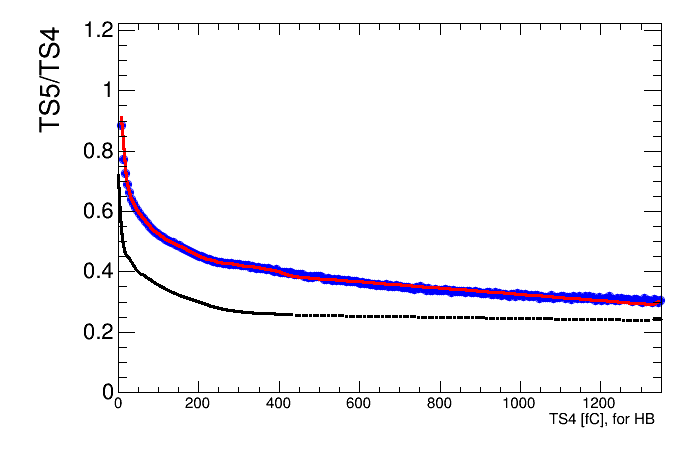
\includegraphics[width=0.6\textwidth]{fig/a1_ring0_daata.png}
%% Text
\label{sec-3-4-4-2}
\begin{itemize}

\item Blue points: MC
\label{sec-3-4-4-2-1}%

\item Red line: MC fit
\label{sec-3-4-4-2-2}%

\item Black line: data fit (from Alexandre)
\label{sec-3-4-4-2-3}%
\end{itemize} % ends low level
\end{frame}
\subsection{a2(TS4) in the QCD sample}
\label{sec-3-5}
\begin{frame}
\frametitle{a2(TS4) in the QCD sample}
\label{sec-3-5-1}
\begin{columns} % Columns
\label{sec-3-5-1-1}
\begin{column}{0.55\textwidth}
%% Figure
\label{sec-3-5-1-1-1}

\centering
a2(TS4) in HB
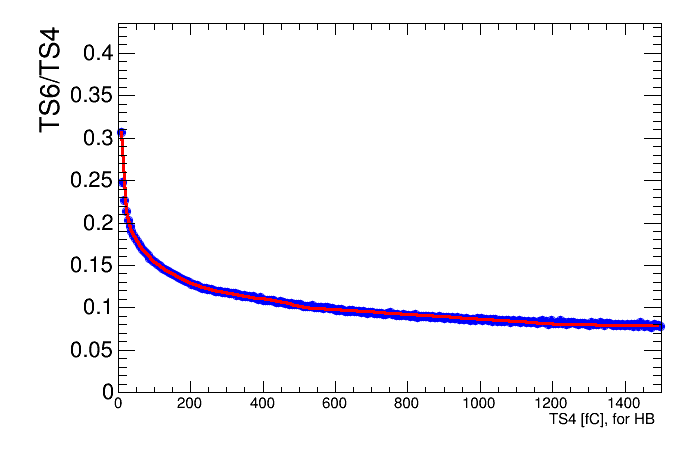
\includegraphics[width=\textwidth]{fig/a2_ring0.png}
\end{column}
\begin{column}{0.55\textwidth}
%% Figure
\label{sec-3-5-1-1-2}

\centering
a2(TS4) in HE 17:20
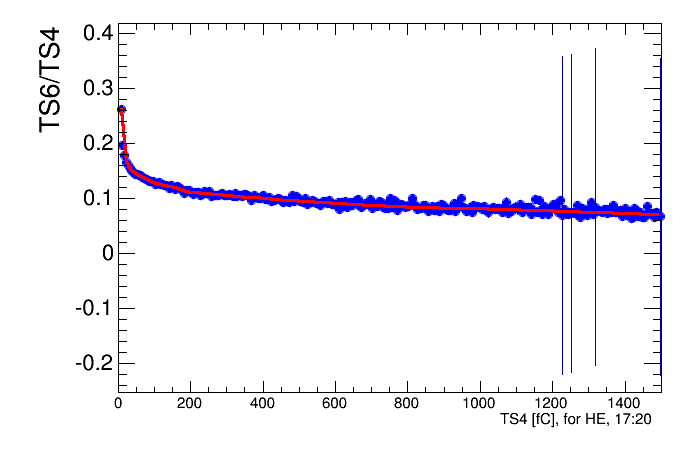
\includegraphics[width=\textwidth]{fig/a2_ring1.png}
\end{column}
\end{columns}
\end{frame}
\begin{frame}
\frametitle{a2(TS4) in the QCD sample: HB}
\label{sec-3-5-2}
%% Table
\label{sec-3-5-2-1}

\begin{center}
\resizebox*{!}{0.75\textheight}{
\begin{tabular}{c|c|rcl|c}
\hline\hline
Variable & Region & \multicolumn{3}{c|}{MC value (unc. from fit)} & Data value \\ 
\hline\hline
$a_{0}$ & \multirow{5}{*}{$\text{TS4} < 23$ fC} & $0.48$ & $\pm$ & $0.00011$ & $0.31$ \\ 
$a_{1}$ & & $-0.03$ & $\pm$ & $7.6e-06$ & $-0.03$ \\ 
$a_{2}$ & & $0.00062$ & $\pm$ & $3.4e-07$ & $0.0017$ \\ 
$a_{3}$ & & $3.7e-05$ & $\pm$ & $1.4e-08$ & $-4.5e-05$ \\ 
$a_{4}$ & & $-1.3e-06$ & $\pm$ & $6e-10$ & $4.4e-07$ \\ 
\hline
$b_{0}$ & \multirow{5}{*}{$23 \leq\text{TS4} < 68$ fC} & $0.26$ & $\pm$ & NA & $0.13$ \\ 
$b_{1}$ & & $-0.0028$ & $\pm$ & $4.1e-06$ & $-0.001$ \\ 
$b_{2}$ & & $1.9e-05$ & $\pm$ & $4.6e-08$ & $1.2e-05$ \\ 
$b_{3}$ & & $2.1e-07$ & $\pm$ & $6.2e-10$ & $-6.7e-08$ \\ 
$b_{4}$ & & $-2.7e-09$ & $\pm$ & $8.6e-12$ & $3.8e-10$ \\ 
\hline
$c_{0}$ & \multirow{4}{*}{$68 \leq\text{TS4} < 190$ fC} & $0.23$ & $\pm$ & NA & $0.11$ \\ 
$c_{1}$ & & $-0.0013$ & $\pm$ & $1.6e-06$ & $-5.3e-05$ \\ 
$c_{2}$ & & $7.1e-06$ & $\pm$ & $6.6e-09$ & $-1.1e-06$ \\ 
$c_{3}$ & & $-1.5e-08$ & $\pm$ & $3e-11$ & $3.7e-09$ \\ 
\hline
$d_{0}$ & \multirow{4}{*}{$190 \leq\text{TS4} < 515$ fC} & $0.19$ & $\pm$ & NA &  $0.1$ \\ 
$d_{1}$ & & $-0.00049$ & $\pm$ & $7.9e-07$  & $-0.00011$ \\ 
$d_{2}$ & & $1.1e-06$ & $\pm$ & $1.2e-09$  & $1.4e-07$ \\ 
$d_{3}$ & & $-1e-09$ & $\pm$ & $2e-12$  & $-7.2e-11$ \\ 
\hline
$e_{0}$ & \multirow{2}{*}{$515 \leq\text{TS4} < 1240$ fC} & $0.11$ & $\pm$ & NA & $0.079$ \\ 
$e_{1}$ & & $-2.8e-05$ & $\pm$ & $1.8e-07$ & $-1.3e-05$ \\ 
\hline
$f_{0}$ & \multirow{2}{*}{$1240 \text{ fC} \leq \text{TS4}$} & $0.11$ & $\pm$ & NA & $0.065$ \\ 
$f_{1}$ & & $-1.8e-06$ & $\pm$ & $8.5e-07$ & $-3.8e-06$ \\ 
\hline\hline
\end{tabular}

}
\end{center}
\end{frame}
\begin{frame}
\frametitle{a2(TS4) in the QCD sample: HE 17:20}
\label{sec-3-5-3}
%% Table
\label{sec-3-5-3-1}

\begin{center}
\resizebox*{!}{0.75\textheight}{
\begin{tabular}{c|c|rcl|c}
\hline\hline
Variable & Region & \multicolumn{3}{c|}{MC value (unc. from fit)} & Data value \\ 
\hline\hline
$a_{0}$ & \multirow{5}{*}{$\text{TS4} < 23$ fC} & $0.47$ & $\pm$ & $0.00052$ & $0.31$ \\ 
$a_{1}$ & & $-0.035$ & $\pm$ & $4.5e-05$ & $-0.027$ \\ 
$a_{2}$ & & $0.00077$ & $\pm$ & $2e-06$ & $0.0014$ \\ 
$a_{3}$ & & $4.4e-05$ & $\pm$ & $8.5e-08$ & $-3.2e-05$ \\ 
$a_{4}$ & & $-1.6e-06$ & $\pm$ & $3.5e-09$ & $2.7e-07$ \\ 
\hline
$b_{0}$ & \multirow{5}{*}{$23 \leq\text{TS4} < 68$ fC} & $0.19$ & $\pm$ & NA & $0.15$ \\ 
$b_{1}$ & & $-0.0013$ & $\pm$ & $2.5e-05$ & $-0.0033$ \\ 
$b_{2}$ & & $3.4e-06$ & $\pm$ & $3e-07$ & $7.8e-05$ \\ 
$b_{3}$ & & $1.6e-07$ & $\pm$ & $4e-09$ & $-9.3e-07$ \\ 
$b_{4}$ & & $-1.3e-09$ & $\pm$ & $5.4e-11$ & $4.5e-09$ \\ 
\hline
$c_{0}$ & \multirow{4}{*}{$68 \leq\text{TS4} < 190$ fC} & $0.19$ & $\pm$ & NA & $0.11$ \\ 
$c_{1}$ & & $-0.0013$ & $\pm$ & $1.1e-05$ & $-0.00025$ \\ 
$c_{2}$ & & $8.3e-06$ & $\pm$ & $4.4e-08$ & $2.9e-07$ \\ 
$c_{3}$ & & $-2e-08$ & $\pm$ & $2e-10$ & $7.7e-10$ \\ 
\hline
$d_{0}$ & \multirow{4}{*}{$190 \leq\text{TS4} < 1000$ fC} & $0.13$ & $\pm$ & NA &  $0.091$ \\ 
$d_{1}$ & & $-7.1e-05$ & $\pm$ & $2.3e-06$  & $-0.0001$ \\ 
$d_{2}$ & & $2e-08$ & $\pm$ & $2.6e-09$  & $1.3e-07$ \\ 
$d_{3}$ & & $8e-12$ & $\pm$ & $2.1e-12$  & $-5.7e-11$ \\ 
\hline
$e_{0}$ & \multirow{2}{*}{$1000 \leq\text{TS4} < 1380$ fC} & $0.1$ & $\pm$ & NA & $0.065$ \\ 
$e_{1}$ & & $-2.1e-05$ & $\pm$ & $2.8e-06$ & $-8.5e-06$ \\ 
\hline
$f_{0}$ & \multirow{2}{*}{$1380 \text{ fC} \leq \text{TS4}$} & $0.1$ & $\pm$ & NA & $0.053$ \\ 
$f_{1}$ & & $-2.7e-05$ & $\pm$ & $1.3e-05$ & $0.0$ \\ 
\hline\hline
\end{tabular}

}
\end{center}
\end{frame}
\begin{frame}
\frametitle{a2(TS4) Data vs QCD MC}
\label{sec-3-5-4}
%% Figure
\label{sec-3-5-4-1}

\centering
a2(TS4) Data vs Monte Carlo in HB
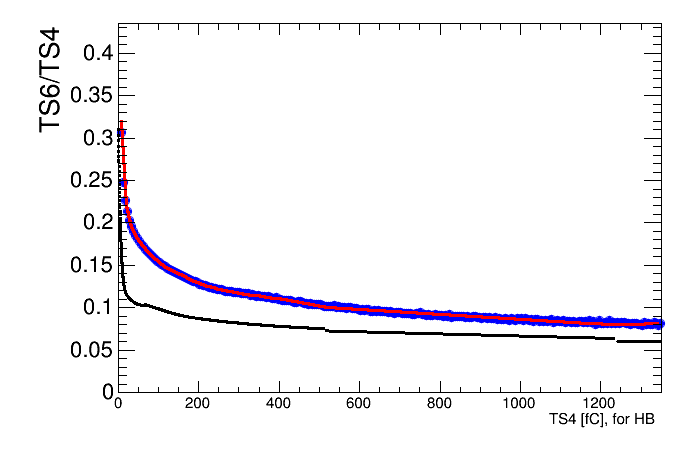
\includegraphics[width=0.6\textwidth]{fig/a2_ring0_daata.png}
%% Text
\label{sec-3-5-4-2}
\begin{itemize}

\item Blue points: MC
\label{sec-3-5-4-2-1}%

\item Red line: MC fit
\label{sec-3-5-4-2-2}%

\item Black line: data fit (from Alexandre)
\label{sec-3-5-4-2-3}%
\end{itemize} % ends low level
\end{frame}
\subsection{a3(TS4) in the QCD sample}
\label{sec-3-6}
\begin{frame}
\frametitle{a3(TS4) in the QCD sample}
\label{sec-3-6-1}
\begin{columns} % Columns
\label{sec-3-6-1-1}
\begin{column}{0.55\textwidth}
%% Figure
\label{sec-3-6-1-1-1}

\centering
a3(TS4) in HB
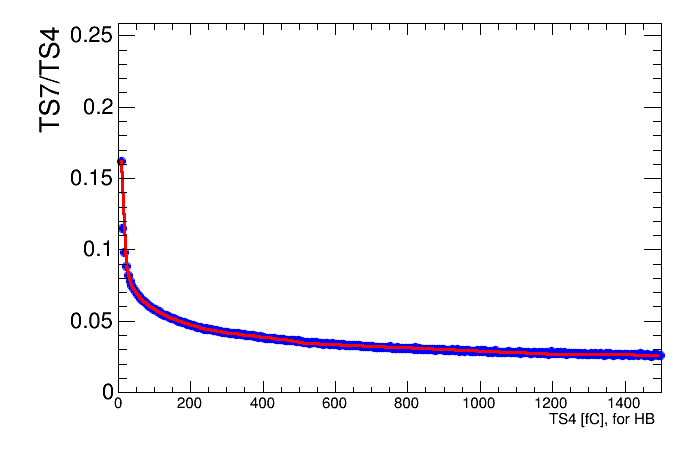
\includegraphics[width=1.0\textwidth]{fig/a3_ring0.png}
\end{column}
\begin{column}{0.55\textwidth}
%% Figure
\label{sec-3-6-1-1-2}

\centering
a3(TS4) in HE 17:20
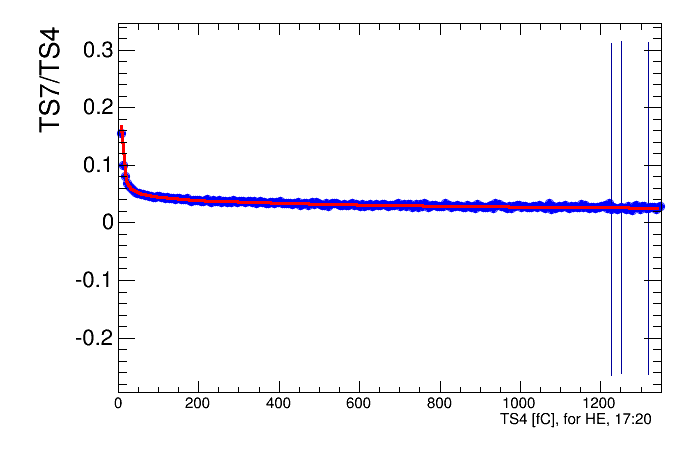
\includegraphics[width=1.0\textwidth]{fig/a3_ring1.png}
\end{column}
\end{columns}
\end{frame}
\begin{frame}
\frametitle{a3(TS4) in the QCD sample: HB}
\label{sec-3-6-2}
%% Table
\label{sec-3-6-2-1}

\begin{center}
\resizebox*{!}{0.75\textheight}{
\begin{tabular}{c|c|rcl|c}
\hline\hline
Variable & Region & \multicolumn{3}{c|}{MC value (unc. from fit)} & Data value \\ 
\hline\hline
$a_{0}$ & \multirow{5}{*}{$\text{TS4} < 23$ fC} & $0.48$ & $\pm$ & $0.00011$ & $0.31$ \\ 
$a_{1}$ & & $-0.03$ & $\pm$ & $7.6e-06$ & $-0.03$ \\ 
$a_{2}$ & & $0.00062$ & $\pm$ & $3.4e-07$ & $0.0017$ \\ 
$a_{3}$ & & $3.7e-05$ & $\pm$ & $1.4e-08$ & $-4.5e-05$ \\ 
$a_{4}$ & & $-1.3e-06$ & $\pm$ & $6e-10$ & $4.4e-07$ \\ 
\hline
$b_{0}$ & \multirow{5}{*}{$23 \leq\text{TS4} < 68$ fC} & $0.26$ & $\pm$ & NA & $0.13$ \\ 
$b_{1}$ & & $-0.0028$ & $\pm$ & $4.1e-06$ & $-0.001$ \\ 
$b_{2}$ & & $1.9e-05$ & $\pm$ & $4.6e-08$ & $1.2e-05$ \\ 
$b_{3}$ & & $2.1e-07$ & $\pm$ & $6.2e-10$ & $-6.7e-08$ \\ 
$b_{4}$ & & $-2.7e-09$ & $\pm$ & $8.6e-12$ & $3.8e-10$ \\ 
\hline
$c_{0}$ & \multirow{4}{*}{$68 \leq\text{TS4} < 190$ fC} & $0.23$ & $\pm$ & NA & $0.11$ \\ 
$c_{1}$ & & $-0.0013$ & $\pm$ & $1.6e-06$ & $-5.3e-05$ \\ 
$c_{2}$ & & $7.1e-06$ & $\pm$ & $6.6e-09$ & $-1.1e-06$ \\ 
$c_{3}$ & & $-1.5e-08$ & $\pm$ & $3e-11$ & $3.7e-09$ \\ 
\hline
$d_{0}$ & \multirow{4}{*}{$190 \leq\text{TS4} < 515$ fC} & $0.19$ & $\pm$ & NA &  $0.1$ \\ 
$d_{1}$ & & $-0.00049$ & $\pm$ & $7.9e-07$  & $-0.00011$ \\ 
$d_{2}$ & & $1.1e-06$ & $\pm$ & $1.2e-09$  & $1.4e-07$ \\ 
$d_{3}$ & & $-1e-09$ & $\pm$ & $2e-12$  & $-7.2e-11$ \\ 
\hline
$e_{0}$ & \multirow{2}{*}{$515 \leq\text{TS4} < 1240$ fC} & $0.11$ & $\pm$ & NA & $0.079$ \\ 
$e_{1}$ & & $-2.8e-05$ & $\pm$ & $1.8e-07$ & $-1.3e-05$ \\ 
\hline
$f_{0}$ & \multirow{2}{*}{$1240 \text{ fC} \leq \text{TS4}$} & $0.11$ & $\pm$ & NA & $0.065$ \\ 
$f_{1}$ & & $-1.8e-06$ & $\pm$ & $8.5e-07$ & $-3.8e-06$ \\ 
\hline\hline
\end{tabular}

}
\end{center}
\end{frame}
\begin{frame}
\frametitle{a3(TS4) in the QCD sample: HE 17:20}
\label{sec-3-6-3}
%% Table
\label{sec-3-6-3-1}

\begin{center}
\resizebox*{!}{0.75\textheight}{
\begin{tabular}{c|c|rcl|c}
\hline\hline
Variable & Region & \multicolumn{3}{c|}{MC value (unc. from fit)} & Data value \\ 
\hline\hline
$a_{0}$ & \multirow{5}{*}{$\text{TS4} < 23$ fC} & $0.47$ & $\pm$ & $0.00052$ & $0.31$ \\ 
$a_{1}$ & & $-0.035$ & $\pm$ & $4.5e-05$ & $-0.027$ \\ 
$a_{2}$ & & $0.00077$ & $\pm$ & $2e-06$ & $0.0014$ \\ 
$a_{3}$ & & $4.4e-05$ & $\pm$ & $8.5e-08$ & $-3.2e-05$ \\ 
$a_{4}$ & & $-1.6e-06$ & $\pm$ & $3.5e-09$ & $2.7e-07$ \\ 
\hline
$b_{0}$ & \multirow{5}{*}{$23 \leq\text{TS4} < 68$ fC} & $0.19$ & $\pm$ & NA & $0.15$ \\ 
$b_{1}$ & & $-0.0013$ & $\pm$ & $2.5e-05$ & $-0.0033$ \\ 
$b_{2}$ & & $3.4e-06$ & $\pm$ & $3e-07$ & $7.8e-05$ \\ 
$b_{3}$ & & $1.6e-07$ & $\pm$ & $4e-09$ & $-9.3e-07$ \\ 
$b_{4}$ & & $-1.3e-09$ & $\pm$ & $5.4e-11$ & $4.5e-09$ \\ 
\hline
$c_{0}$ & \multirow{4}{*}{$68 \leq\text{TS4} < 190$ fC} & $0.19$ & $\pm$ & NA & $0.11$ \\ 
$c_{1}$ & & $-0.0013$ & $\pm$ & $1.1e-05$ & $-0.00025$ \\ 
$c_{2}$ & & $8.3e-06$ & $\pm$ & $4.4e-08$ & $2.9e-07$ \\ 
$c_{3}$ & & $-2e-08$ & $\pm$ & $2e-10$ & $7.7e-10$ \\ 
\hline
$d_{0}$ & \multirow{4}{*}{$190 \leq\text{TS4} < 1000$ fC} & $0.13$ & $\pm$ & NA &  $0.091$ \\ 
$d_{1}$ & & $-7.1e-05$ & $\pm$ & $2.3e-06$  & $-0.0001$ \\ 
$d_{2}$ & & $2e-08$ & $\pm$ & $2.6e-09$  & $1.3e-07$ \\ 
$d_{3}$ & & $8e-12$ & $\pm$ & $2.1e-12$  & $-5.7e-11$ \\ 
\hline
$e_{0}$ & \multirow{2}{*}{$1000 \leq\text{TS4} < 1380$ fC} & $0.1$ & $\pm$ & NA & $0.065$ \\ 
$e_{1}$ & & $-2.1e-05$ & $\pm$ & $2.8e-06$ & $-8.5e-06$ \\ 
\hline
$f_{0}$ & \multirow{2}{*}{$1380 \text{ fC} \leq \text{TS4}$} & $0.1$ & $\pm$ & NA & $0.053$ \\ 
$f_{1}$ & & $-2.7e-05$ & $\pm$ & $1.3e-05$ & $0.0$ \\ 
\hline\hline
\end{tabular}

}
\end{center}
\end{frame}
\begin{frame}
\frametitle{a3(TS4) Data vs QCD MC}
\label{sec-3-6-4}
%% Figure
\label{sec-3-6-4-1}

\centering
a3(TS4) Data vs Monte Carlo in HB
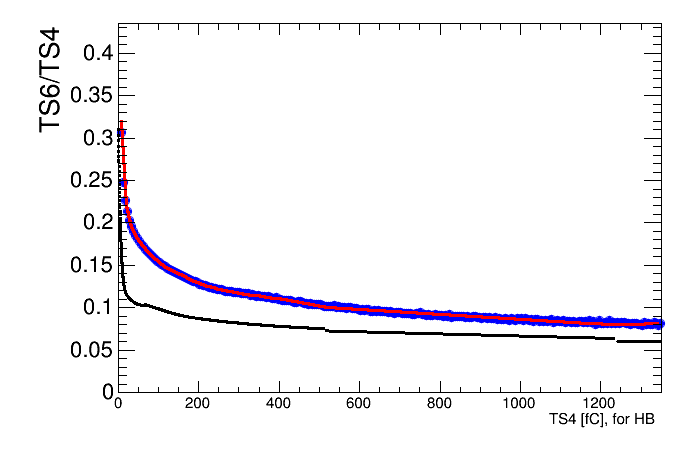
\includegraphics[width=0.6\textwidth]{fig/a2_ring0_daata.png}
%% Text
\label{sec-3-6-4-2}
\begin{itemize}

\item Blue points: MC
\label{sec-3-6-4-2-1}%

\item Red line: MC fit
\label{sec-3-6-4-2-2}%

\item Black line: data fit (from Alexandre)
\label{sec-3-6-4-2-3}%
\end{itemize} % ends low level
\end{frame}
\section{Conclusion}
\label{sec-4}
\subsection{Conclusion}
\label{sec-4-1}
\begin{frame}
\frametitle{Conclusion}
\label{sec-4-1-1}
\begin{itemize}

\item Processed zero-pileup samples adequate for studies
\label{sec-4-1-1-1}%

\item Preliminary results ready using Alexandre's method
\label{sec-4-1-1-2}%
\begin{itemize}

\item Fit functions used for data model MC pulse shape well
\label{sec-4-1-1-2-1}%

\item Final fit parameters (i.e. pulse shapes) are significantly different between data and MC
\label{sec-4-1-1-2-2}%
\end{itemize} % ends low level

\item Working on validating results to put into CMSSW in time for 710
\label{sec-4-1-1-3}%
\end{itemize} % ends low level
\end{frame}

\end{document}
